\section{Neural Networks and Deep Learning}


\subsection{Convolutional Neural Networks CNN}

A convolutional neural network is a deep learning algorithm which is primarily used to classify images. It can more easily capture spatial (and temporal) dependencies since the convolution filters use a linear combination of neighboring pixels to calculate an output value. After a convolution filter is applied, a max-pooling filter can be applied, which lowers the amount of nodes in the network. A $2$x$2$ max-pooling filter, for example, replaces every $2$x$2$ square with the maximal value in that square, resulting in lowering the amount of nodes after that layer to a quarter.
At the end the multidimensional layers are flattened to a one dimensional vector that is connected to the output via a fully connected layer.

\begin{figure}[hbtp]
	\centering
	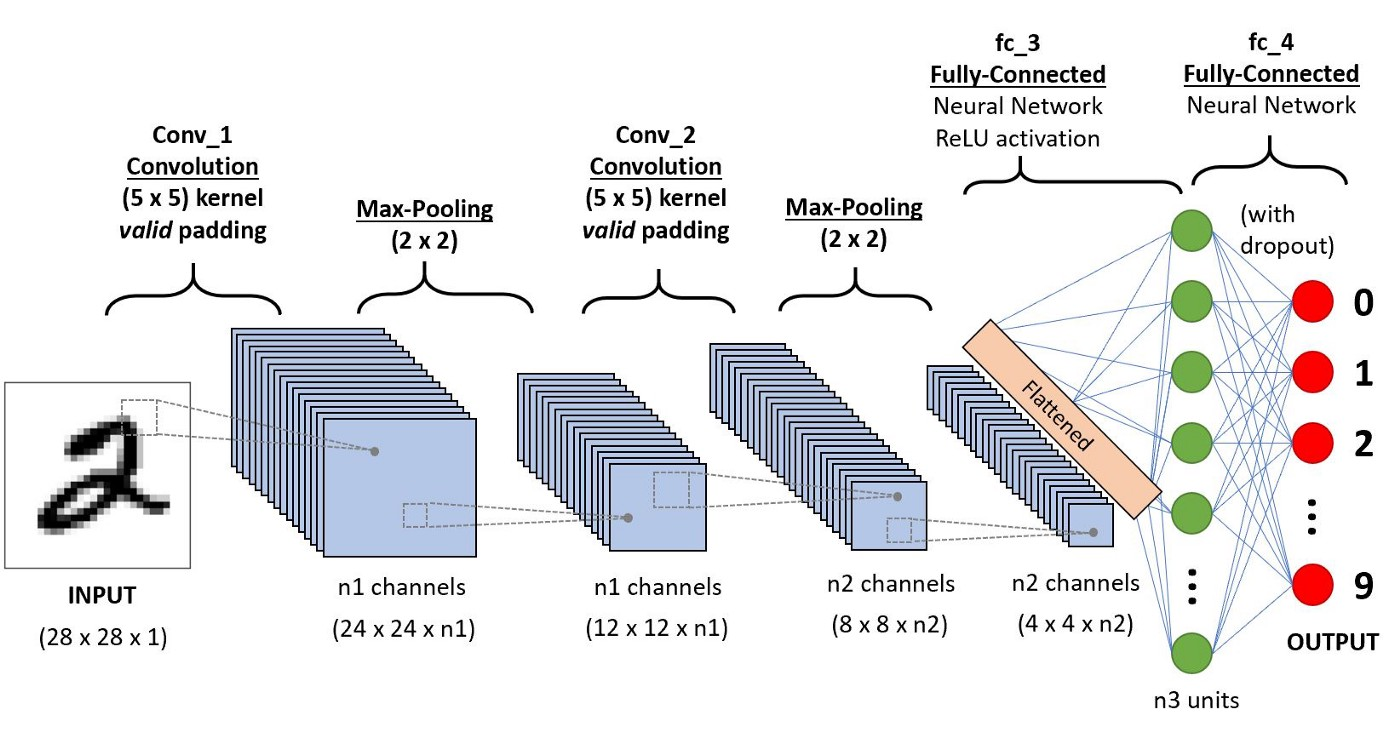
\includegraphics[width=1\textwidth]{Images/CNN}
	\caption{Example of a CNN architecture}
\end{figure}

Helpful links:\\
A Comprehensive Guide to Convolutional Neural Networks — the ELI5 way
\\
\url{https://towardsdatascience.com/a-comprehensive-guide-to-convolutional-neural-networks-the-eli5-way-3bd2b1164a53}
\\

Since we want to detect emotions in images, a convolutional neural network would be a good choice. It is the go-to type of network for these kind of computer vision problems.

\subsection{Recurrent Neural Networks RNN}

A recurrent neural network (RNN) is a type of artificial neural network commonly used in speech recognition and natural language processing. It uses feedback loops, that allow information to persist (the network has memory), to process sequences of data.\\

RNNs are not useful to analyse facial expression in an image.

\subsection{Generative adversarial networks GAN}

Generative adversarial networks (GANs) are algorithmic architectures that use two neural networks, pitting one against the other in order to generate new, synthetic instances of data that can pass for real data. They are used widely in image generation, video generation and voice generation.\\
One neural network, called the generator, generates new data instances, while the other, the discriminator, evaluates them for authenticity; i.e. the discriminator decides whether each instance of data that it reviews belongs to the actual training dataset or not.\\

Helpful links:\\
A Beginner's Guide to Generative Adversarial Networks (GANs)
\\
\url{https://pathmind.com/wiki/generative-adversarial-network-gan}
\\

GANs can be used to generate images and videos. We could use this type of network to expand training data. 
Having a well trained GAN would allow us to create new images for specific emotions that look convincingly real in order to prevent overfitting by creating an almost endless stream of new images. 
It may also be used to create video training data that can be used to train a neural network with memory to better capture changes in emotion in a video stream. 
The training of a GAN however takes a very long time compared to a simple CNN which makes it probably unfeasible for us even though it would create interesting possibilities to explore. 


\subsection{Autoencoders}

Autoencoders are a specific type of feedforward neural networks where the input is the same as the output. They compress the input into a lower-dimensional code and then reconstruct the output from this representation. The code is a compact “summary” or “compression” of the input.
An autoencoder consists of 3 components: encoder, code and decoder. The encoder compresses the input and produces the code, the decoder then reconstructs the input only using this code.\\

Helpful links:\\
Applied Deep Learning - Part 3: Autoencoders
\\
\url{https://towardsdatascience.com/applied-deep-learning-part-3-autoencoders-1c083af4d798}\\

An autoencoder is used to reduce the dimensionality. Since there is a lot of redundancy in images, especially if they all contain more or less centered faces, it can be expected that an autoencoder could shrink the input size considerably before using a different neural network. This could potentially make the training process a lot quicker. We would however not be able to use a convolutional neural network anymore because the 2 dimensional image structure is lost by removing the redundancy with the autoencoder. Moreover some information may be lost in the process which could affect the overall accuracy of the neural network. 

The effectiveness of an autoencoder could possibly be explored if there are given time constraints for the training process. It can also be compared to principal component analysis (PCA) which removes redundancy in a more controlled way. 

\begin{figure}[hbtp]
	\centering
	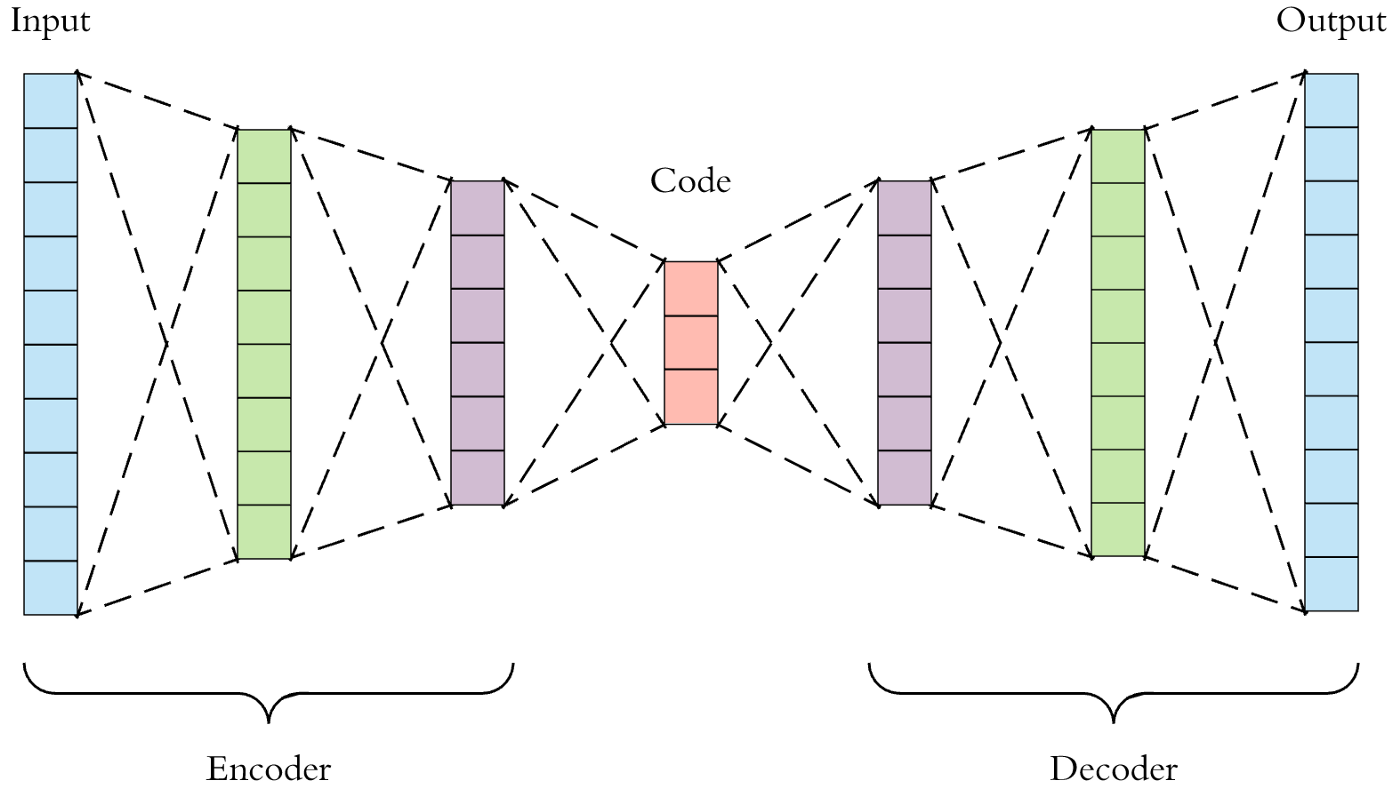
\includegraphics[width=1\textwidth]{Images/Autoencoder}
	\caption{Example of an autoencoder architecture}
\end{figure}


\subsection{Perceptrons MLP}


%%%%%%%%%%%%%%%%%%%%%%%%%%%%%%%%%%%%%%%%%%%%%%%%%%%%%%%%%


\newpage